\documentclass[11pt]{article}

% paper.tex builds the anonymous review version; preprint.tex defines \preprintmode and builds the arXiv version.
\ifdefined\preprintmode
\usepackage[preprint]{acl}
\else
\usepackage[review]{acl}
\fi

\usepackage{times}
\usepackage{latexsym}
\usepackage[T1]{fontenc}
\usepackage[utf8]{inputenc}
\usepackage{microtype}
\usepackage{inconsolata}
\usepackage{graphicx}
\usepackage{booktabs}
\usepackage{multirow}
\usepackage{amsmath}
\usepackage{amssymb}
\usepackage{algorithm}
\usepackage{algpseudocode}
\usepackage{xspace}
\usepackage{float}

\newcommand{\candGapN}{45}
\newcommand{\candGapRho}{0.28}
\newcommand{\cladePooledGain}{+0.05 [$-$0.01, +0.11]}
\newcommand{\cladePooledGainP}{0.062}
\newcommand{\cladeSdGain}{+0.13 [+0.01, +0.27]}
\newcommand{\harmAce}{1/9}
\newcommand{\harmClade}{0/9}
\newcommand{\harmGepa}{4/9}
\newcommand{\harmGepatools}{4/9}
\newcommand{\harmMipro}{2/9}
\newcommand{\nWriteAir}{13}
\newcommand{\nWriteRet}{36}
\newcommand{\retVsAce}{+0.06 [$-$0.01, +0.12]}
\newcommand{\retVsGepa}{+0.10 [$-$0.00, +0.20]}
\newcommand{\retVsGepatools}{+0.12 [+0.03, +0.22]}
\newcommand{\retVsMipro}{+0.08 [+0.01, +0.15]}
\newcommand{\sdVsAce}{+0.16 [+0.03, +0.33]}
\newcommand{\sdVsAceP}{0.014}
\newcommand{\sdVsGepa}{+0.24 [+0.08, +0.42]}
\newcommand{\sdVsGepaP}{0.004}
\newcommand{\sdVsGepatools}{+0.29 [+0.11, +0.47]}
\newcommand{\sdVsGepatoolsP}{0.002}
\newcommand{\sdVsMipro}{+0.18 [$-$0.06, +0.54]}
\newcommand{\sdVsMiproP}{0.172}
\newcommand{\sizeAceMax}{64{,}636}
\newcommand{\sizeAceMin}{15{,}876}
\newcommand{\sizeCladeMax}{710}
\newcommand{\sizeCladeMin}{306}
\newcommand{\startAirMax}{0.54}
\newcommand{\startAirMean}{0.46}
\newcommand{\startAirMin}{0.38}
\newcommand{\startAirN}{16}
\newcommand{\startRetMax}{0.54}
\newcommand{\startRetMean}{0.48}
\newcommand{\startRetMin}{0.44}
\newcommand{\startRetN}{6}
\newcommand{\startSupMax}{0.76}
\newcommand{\startSupMean}{0.75}
\newcommand{\startSupMin}{0.74}
\newcommand{\startSupN}{3}

\newcommand{\clade}{\textsc{Clade}\xspace}
\newcommand{\taub}{$\tau^2$-bench\xspace}

\title{Prompt Optimizers Can Make Tool-Using Agents Worse:\\An Equal-Budget Study and a Gated Alternative}

\ifdefined\preprintmode
\author{Kumar Ashish \\
  Harvard Extension School, Harvard University \\
  \texttt{kua613@g.harvard.edu}}
\else
\author{Anonymous ACL submission}
\fi

\begin{document}
\maketitle

\begin{abstract}
Prompt and context optimizers such as GEPA, MIPROv2 and ACE improve language-model systems by rewriting their
instructions from execution feedback, and are increasingly applied to tool-using agents. Their reported gains come
from comparisons run by their authors, on their own tasks, usually with one run per configuration. We compare them
under one harness: the same agent (gpt-oss-20b), reflection model, practice tasks, episode rendering and rollout
budget, a frozen test split, three seeds, and a protocol fixed before the main runs. On \taub airline and retail, no
optimizer reliably improves the agent within 600 rollouts, while the test score of the unchanged agent alone varies
from \startAirMin{} to \startAirMax{} between scorings. The competitors often ship a worse agent: GEPA's and
MIPROv2's shipped agents score below every scoring of the unchanged agent in \harmGepa{} and \harmMipro{} of their
runs, one of them with a rewritten prompt that told the agent to type its tool calls as JSON text. We introduce \clade, which edits one component at a time (a rule, a prompt section or a
tool description), screens proposed fixes for task-specific content, and promotes a change only if it wins on
held-out tasks without a per-task drop larger than run-to-run noise. \clade never shipped a harmful agent
(\harmClade{} runs), was ahead of every competitor on retail (significantly against one of four after correction, marginally against a
second), improved the agent
on a development benchmark by \cladeSdGain{}, and was the cheapest and fastest method. Its own gain on \taub is small
and not significant, and our ablations do not isolate a single component. We release the harness, protocol and all
runs.
\end{abstract}

\section{Introduction}

When an agent's weights cannot be changed (a closed model, or a deployment where fine-tuning is too costly), the
remaining lever is what the model is told: its system prompt, any learned rules, and the descriptions of its tools.
A family of optimizers edits these automatically from the agent's own executions. MIPROv2 proposes and searches over
instructions \citep{mipro}; TextGrad backpropagates textual critiques \citep{textgrad}; GEPA reflects on trajectories
and evolves prompts with a Pareto archive \citep{gepa}; ACE grows a playbook of strategies from reflections
\citep{ace}. These methods report gains of several to tens of points, and some ship in widely used frameworks
\citep{dspy}.

Two features of tool-using agents make those gains hard to transfer. First, agents are stochastic: the same agent on
the same task can pass on one run and fail on the next, so a candidate prompt's score on a small validation set is
noisy. Second, practice tasks are few: a team with a working agent rarely has hundreds of verified tasks. An
optimizer that selects the best of many candidates on a noisy, small validation set will often select noise, and the
prompt it ships can be worse than the one it started from. For a practitioner, that is the outcome that matters most:
an optimizer that sometimes makes a working agent worse cannot be run unattended.

We test this directly. We build one harness in which every optimizer drives the same agent through the same counted
rollout path, reads the same rendering of each episode, uses the same reflection model and practice tasks, and has
its shipped agent scored on the same frozen test split, with three seeds and a protocol fixed before the main runs
(\S\ref{sec:setup}). We also introduce \clade (\S\ref{sec:method}), an optimizer designed around the failure mode
above: it proposes one bounded change at a time, screens proposed fixes before spending episodes on them, and
promotes a change only through a held-out gate that tolerates run-to-run noise but no larger per-task drop.

Our findings (\S\ref{sec:results}):
\begin{itemize}
\setlength\itemsep{0pt}
\item On \taub airline and retail with a gpt-oss-20b agent, no optimizer reliably improves the agent within 600
rollouts. The unchanged agent's test score varies by up to 0.16 between scorings, more than most reported gains.
\item The competitors frequently ship a worse agent. Across 9 runs each, the shipped agent
scored below every scoring of the starting agent in \harmGepa{} runs for GEPA, \harmGepatools{} for GEPA with tool
descriptions, \harmMipro{} for MIPROv2 and \harmAce{} for ACE.
\item \clade never shipped a harmful agent (\harmClade{}). On retail it is ahead of every competitor, significantly
against GEPA with tool descriptions and marginally against MIPROv2 after Holm correction. On our development benchmark it improves the
agent by \cladeSdGain{}. It is the cheapest and fastest method per run.
\item The protection comes mostly from declining to change the agent: \clade shipped the starting agent unchanged in
three of six \taub runs, and its own gain over the starting agent on \taub is small (\cladePooledGain{}). No single
component's removal significantly hurts.
\end{itemize}

\section{Related work}

\paragraph{Prompt optimization.} APE \citep{ape} and OPRO \citep{opro} generate and score candidate instructions;
Promptbreeder evolves prompts and the mutation prompts that produce them \citep{promptbreeder}. DSPy \citep{dspy}
compiles language-model programs, with MIPROv2 \citep{mipro} searching instructions and demonstrations by Bayesian
optimization and SIMBA \citep{simba} adding rules from contrasting trajectories. TextGrad \citep{textgrad} and Trace
\citep{trace} treat textual feedback as a gradient. GEPA \citep{gepa} reflects on trajectories in natural language and
keeps a Pareto front of candidates, and reports outperforming reinforcement learning with far fewer rollouts.
\citet{beyondprompts} compare GEPA and MIPROv2 on \taub at matched rollouts and find GEPA's prompt-only gains on
retail negative; \citet{textreg} describe prompt overfitting, where narrow, sample-specific rules accumulate as
training loss falls.

\paragraph{Learning from experience.} Reflexion \citep{reflexion} turns failures into verbal feedback within a task;
ExpeL \citep{expel}, Agent Workflow Memory \citep{awm}, Dynamic Cheatsheet \citep{dynamiccheatsheet} and
ReasoningBank \citep{reasoningbank} accumulate reusable insights across tasks. ACE \citep{ace} curates an evolving
playbook through generator, reflector and curator roles with incremental updates. \clade shares the
reflect-and-curate structure; it differs in bounding each change, screening fixes before evaluation, and gating
promotion on held-out tasks.

\paragraph{Self-improving agents.} The Darwin G\"odel Machine \citep{dgm} keeps an archive of self-modified agents;
the Huxley-G\"odel Machine \citep{hgm} chooses which agent to expand by the success of its descendants (clade
metaproductivity), which \clade uses to choose parents among bundle versions. Meta-Harness \citep{metaharness}
searches over harness code. Concerns about evaluation in this area, including cost, reproducibility and held-out
splits, are summarized by \citet{agentsthatmatter}; our protocol follows their recommendations.

\section{\clade}
\label{sec:method}

\clade optimizes a \emph{bundle}: the agent's system prompt, a list of playbook rules rendered into it, and
overrides for tool descriptions. Every candidate is a versioned child of a parent bundle with the diagnosis that
produced it, so any promoted change can be traced to the failures it fixed. The model's weights never change.

\begin{algorithm}[t]
\caption{One \clade round}
\label{alg:clade}
\small
\begin{algorithmic}[1]
\State plan lanes: the incumbent, then archive parents by clade score, else the incumbent under another lens
\For{each lane with parent $P$ (in parallel)}
  \State $D \gets$ \textsc{Reflect}(failed training episodes of $P$)
  \State $D \gets$ \textsc{Critic}($D$, playbook of $P$)
  \State $C_P \gets$ \textsc{Curate}($P$, $D$) \Comment{bounded edits}
\EndFor
\For{each candidate $c$, while the budget allows one more evaluation}
  \State run $c$ $n$ times on every training and held-out task
\EndFor
\State $c^\star \gets \arg\max_c\, (\bar s_{\mathrm{held}}(c), \bar s_{\mathrm{train}}(c))$
\If{$c^\star$ beats the incumbent \textbf{and} $\max_t [s_{\mathrm{inc}}(t) - s_{c^\star}(t)] \le \max(\delta, 1/n)$}
  \State promote $c^\star$
\EndIf
\end{algorithmic}
\end{algorithm}

\paragraph{Reflector.} For a parent bundle, the reflector reads its failed episodes on \emph{training} tasks (never
held-out ones): one diagnosis per failing task (up to four) and one cross-cutting diagnosis across tasks, each with
the root process mistake and one general fix. Each episode is rendered as its trajectory, final reply and the
judge's verdict, trimmed in the middle when long. A fix that quotes code or names an identifier seen in the
episode's tool traffic is discarded as task-specific.

\paragraph{Critic.} One further model call reviews the surviving fixes and drops those that are hints about one task,
not actionable, or already said by the playbook. Fixes are screened before any episode is spent on them.

\paragraph{Curator.} Each fix becomes a bounded candidate that changes one component: a single playbook rule (the
fix itself, deduplicated against existing rules by a yes/no model call, at most eight rules); one appended prompt
section of at most six lines; or a rewrite of one tool's description (at most 400 characters, no identifiers), when a
diagnosis concerns tool use. A further candidate combines the round's new rules. Whole-prompt rewrites are never
proposed.

\paragraph{Selector and gate.} Each candidate is run $n$ times on every training and held-out task. The candidate
with the best held-out mean (training mean as tie-break) is promoted only if it beats the incumbent and no task's
mean drops by more than $\max(\delta, 1/n)$, with $\delta = 0.34$. With $n=2$, one extra failed run on a task is
tolerated as noise; a larger drop blocks promotion. Training episodes of a promoted candidate become the next
round's material for reflection.

\paragraph{Coordinator and archive.} Every evaluated version enters an archive. Each round runs up to three lanes in
parallel: the incumbent, and the archive's best parents by clade score (mean held-out score of a node's descendants)
plus an exploration bonus $c\sqrt{\ln N/(1+k)}$, where $N$ is the archive size and $k$ the node's number of children
\citep{hgm}. When the archive has no second parent, extra lanes reread the incumbent's failures through a different
lens (contrast with a success; tool use only). The run stops after three rounds, after two rounds without a
promotion, or when the rollout budget cannot cover another evaluation with room to spare.

\section{Experimental setup}
\label{sec:setup}

\paragraph{Benchmarks.} \taub \citep{tau2bench} (v1.0.1) simulates customer service: an agent with domain tools and a
written policy talks to a simulated user, and is scored 1 only if the final database state matches the expected
outcome and, where a task requires it, the agent told the user the required information (airline) or satisfied
natural-language assertions checked by a judge (retail). We use the airline and retail domains. Practice tasks are
20 training and 10 validation tasks drawn once from each domain's official train split; the test split is the
official one (20 airline, 40 retail tasks), each test task run 4 times. The agent is \taub's own LLM agent; a bundle
replaces only its instruction block and may override tool descriptions, and the domain policy is passed verbatim, so
the starting bundle \emph{is} \taub's default agent. The user simulator and retail's assertion judge are gpt-oss-120b
at temperature 0. Our \emph{support desk} is a smaller customer-support environment (9 tools, a refund and
cancellation policy, scored by hidden tests on the store's side effects) with 7 training, 3 validation and 20 test
tasks, each run 10 times. \clade was developed on it, so we report it as a development benchmark only.

\paragraph{Models.} The agent is gpt-oss-20b \citep{gptoss}. Every optimizer uses gpt-oss-120b for reflection,
proposal and curation.

\paragraph{Competitors.} We use each method's official library where one exists and its default configuration sized
to the budget: GEPA (\texttt{gepa} 0.1.4, reflective proposer, minibatch 3), once on the system prompt only, as in its
experiments, and once with every tool description as an additional component (GEPA+tools), the same search space
\clade edits; MIPROv2 (DSPy 3.4.0, instruction only, trials sized to the budget); and ACE, ported from the official
prompts and code (temperature 0, up to three reflection rounds per task, up to five epochs, best epoch on
validation). Appendix~\ref{app:config} lists every setting.

\paragraph{Equal treatment.} Every method runs the agent only through the harness, which counts one rollout per
episode; an episode lost to the provider is re-run and counted once. All methods read the same rendering of an
episode, evaluate validation tasks twice, and receive 600 rollouts per run on \taub (400 on the support desk). No
method sees a test task. A shipped agent is scored on the test split in a separate store.

\paragraph{Protocol and statistics.} Hypotheses, splits, budgets, seeds and analysis were fixed before the main runs;
three deviations made before any \taub result existed (a lower budget, a reduced scope, and a bug fix in the ACE port)
are listed in Appendix~\ref{app:protocol}. Each method has three seeds per benchmark, and the starting agent is scored
three times. Intervals are 95\% hierarchical bootstraps that resample test tasks and then each method's seeds
\citep{efron}. Comparisons of \clade with the four competitors are Holm-corrected within each benchmark \citep{holm}.

\begin{table*}[t]
\centering
\small
\begin{tabular}{lcccccccc}
\toprule
& \multicolumn{2}{c}{\taub airline} & \multicolumn{2}{c}{\taub retail} & \multicolumn{2}{c}{Support desk (dev.)} & \multicolumn{2}{c}{Cost per \taub run} \\
\cmidrule(lr){2-3}\cmidrule(lr){4-5}\cmidrule(lr){6-7}\cmidrule(lr){8-9}
Method & score & $\Delta$ (changed) & score & $\Delta$ (changed) & score & $\Delta$ (changed) & USD & hours \\
\midrule
Starting agent & 0.433 & -- & 0.475 & -- & 0.748 & -- & -- & -- \\
\textsc{Clade} & 0.467 & +0.033 \scriptsize(1/3) & 0.533 & +0.058 \scriptsize(2/3) & 0.882 & +0.133 \scriptsize(3/3) & 3.31 & 2.5 \\
GEPA & 0.467 & +0.033 \scriptsize(0/3) & 0.438 & $-$0.037 \scriptsize(3/3) & 0.640 & $-$0.108 \scriptsize(3/3) & 4.49 & 6.7 \\
GEPA+tools & 0.425 & $-$0.008 \scriptsize(2/3) & 0.410 & $-$0.065 \scriptsize(2/3) & 0.587 & $-$0.162 \scriptsize(3/3) & 5.12 & 7.0 \\
MIPROv2 & 0.479 & +0.046 \scriptsize(0/3) & 0.454 & $-$0.021 \scriptsize(2/3) & 0.702 & $-$0.047 \scriptsize(3/3) & 3.86 & 3.5 \\
ACE & 0.442 & +0.008 \scriptsize(3/3) & 0.475 & +0.000 \scriptsize(3/3) & 0.723 & $-$0.025 \scriptsize(3/3) & 4.68 & 8.2 \\
\bottomrule

\end{tabular}
\caption{Test score (mean of three seeds), difference from the starting agent, and in brackets the number of runs whose
shipped agent differs from the starting one. Cost is learning cost per run (optimizer calls and learning episodes,
at list prices) and wall-clock learning time, averaged over the \taub runs.}
\label{tab:main}
\end{table*}

\begin{figure*}[t]
\centering
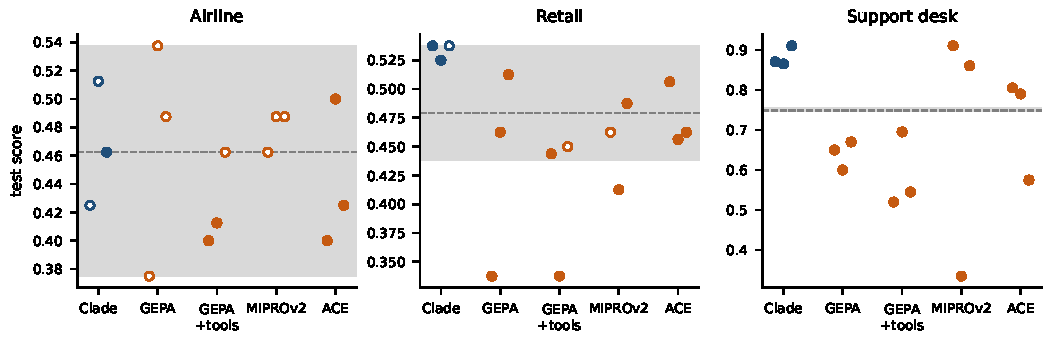
\includegraphics[width=\textwidth]{figures/runs.pdf}
\caption{Every run's test score. The grey band spans all scorings of the unchanged starting agent (\startAirN{} on
airline, \startRetN{} on retail, \startSupN{} on the support desk) and the dashed line is their mean. Hollow markers
are runs that shipped the starting agent unchanged; their spread is scoring noise.}
\label{fig:runs}
\end{figure*}

\section{Results}
\label{sec:results}

\paragraph{No optimizer reliably improves the agent on \taub.} Table~\ref{tab:main} gives the scores. On airline the
methods span 0.425 to 0.479 against 0.433 for the starting agent, and none differs significantly from it or from
\clade (Table~\ref{tab:vs}). On retail, only \clade is above the starting agent. Pooled over both domains, \clade's
gain over the starting agent is \cladePooledGain{} ($p=\cladePooledGainP$). The scale of these differences should be
read against scoring noise: across all scorings of the \emph{unchanged} starting agent, including runs that shipped it
unchanged, its test score ranged from \startAirMin{} to \startAirMax{} on airline and from \startRetMin{} to
\startRetMax{} on retail (Figure~\ref{fig:runs}). GEPA and MIPROv2 shipped the unchanged starting prompt in all three
airline runs, so their airline scores (0.467 and 0.479) are re-scorings of the starting agent. Airline is hard for
this agent: on the \nWriteAir{} test tasks that need a database write, every method scores between 0.17 and 0.28
(Appendix~\ref{app:size}).

\paragraph{Optimizers often ship a worse agent.} We call a run harmful when its shipped agent scores below \emph{every}
scoring of the unchanged starting agent on the same benchmark. Out of nine runs per method (three seeds on three
benchmarks), GEPA had \harmGepa{} harmful runs, GEPA+tools \harmGepatools{}, MIPROv2 \harmMipro{}, ACE \harmAce{} and
\clade \harmClade{}. The worst shipped agents scored 0.338 on retail (against 0.44 to 0.54 for the starting agent)
and 0.335 on the support desk (against 0.74 to 0.76). The overfitting gap (validation score of the shipped bundle
minus its test score; Appendix Table~\ref{tab:seeds}) shows why: on retail and the support desk, GEPA's and
GEPA+tools' shipped prompts scored 0.17 to 0.36 higher on their validation tasks than on test, \clade's 0.02 and 0.12. One MIPROv2 prompt on the support desk
addressed only the single customer who appears in the practice tasks and quoted task identifiers
(Appendix~\ref{app:examples}). Giving GEPA the tool descriptions as well (GEPA+tools) did not help: a larger search
space with the same selection overfit further. The gap is only weakly associated with the number of candidates a
run compared on its validation tasks (Spearman $\rho=\candGapRho$ over \candGapN{} runs), so multiple comparisons
alone do not explain it; what a candidate changes matters too.

\paragraph{What the harmful prompts contain.} GEPA's worst retail prompt (test score 0.338) rewrote \taub's
two-paragraph instruction into a 6{,}000-character prompt whose first rule reads: ``on every turn you must output
exactly one of the following JSON objects and nothing else'', followed by templates such as
\texttt{\{"type": "tool", "name": ..., "arguments": ...\}}. It reinterprets \taub's request to ``generate valid
JSON'' as an instruction to write tool calls as text, which conflicts with the model's native tool calling; the agent
then attempted calls to a non-existent tool named \texttt{json}. Such rewrites change how the agent interacts, not
what it knows, and a few validation tasks cannot reveal the damage. ACE's failure mode is different: its playbooks
grew to between \sizeAceMin{} and \sizeAceMax{} characters on \taub, about 50 to 210 times the starting instruction, a
cost every later episode pays, for no gain on test. \clade's shipped prompts stayed between \sizeCladeMin{} and
\sizeCladeMax{} characters.

\begin{table}[t]
\centering
\small
\setlength{\tabcolsep}{3pt}
\begin{tabular}{lcc}
\toprule
Competitor & Airline & Retail \\
\midrule
GEPA & +0.00 [$-$0.10, +0.11] & +0.10 [$-$0.00, +0.20] \\
 & {\scriptsize $p=1.000$} & {\scriptsize $p=0.067$} \\
GEPA+tools & +0.04 [$-$0.03, +0.13] & +0.12 [+0.03, +0.22] \\
 & {\scriptsize $p=0.660$} & {\scriptsize $p=0.026$} \\
MIPROv2 & $-$0.01 [$-$0.10, +0.07] & +0.08 [+0.01, +0.15] \\
 & {\scriptsize $p=1.000$} & {\scriptsize $p=0.041$} \\
ACE & +0.03 [$-$0.09, +0.15] & +0.06 [$-$0.01, +0.12] \\
 & {\scriptsize $p=1.000$} & {\scriptsize $p=0.067$} \\
\bottomrule

\end{tabular}
\caption{\clade minus competitor on \taub test score, with 95\% intervals and Holm-adjusted one-sided $p$ (below).
Positive favours \clade. Pooled results are in Appendix~\ref{app:pooled}.}
\label{tab:vs}
\end{table}

\paragraph{\clade against the competitors.} Table~\ref{tab:vs} compares \clade with each competitor. On retail
\clade is ahead of all four: significantly against GEPA+tools (\retVsGepatools{}) after Holm correction, marginally
against MIPROv2 (\retVsMipro{}; its Holm-adjusted $p$ ranges from 0.037 to 0.050 across ten bootstrap seeds), and
with $p\approx0.07$ against GEPA and ACE. On airline all differences are within $\pm0.05$ and none is
significant. On the development benchmark \clade is ahead of GEPA (\sdVsGepa{}), GEPA+tools (\sdVsGepatools{}) and
ACE (\sdVsAce{}), all significant, and of MIPROv2 by \sdVsMipro{}, not significant because one MIPROv2 seed collapsed.

\paragraph{What \clade changed.} Each \clade run on \taub evaluated eight candidates, and the selector rejected most:
\clade shipped the unchanged agent in two of three airline runs and one of three retail runs. In three of the six
runs the candidate with the best held-out mean was blocked by the per-task gate because one held-out task dropped
from always passing to always failing. Each changed bundle added a single prompt section, for
example, on retail, ``After confirming the user's identity, you must invoke the appropriate domain-specific tool
(exchange, cancel, modify, return) before ending the turn. Do not end the conversation or transfer to a human unless
the tool call fails or the user explicitly asks.'' The two changed retail bundles scored 0.537 and 0.525. On the
support desk all three runs changed the agent and all three improved it (0.865 to 0.910 against 0.74 to 0.76). Its
protection on \taub is therefore mostly a matter of not shipping changes that do not clearly win, rather than of
finding better prompts.

\paragraph{Cost.} \clade was the cheapest and fastest method per run (Table~\ref{tab:main}). Its
critic discards fixes before they cost episodes, and each candidate's episodes run in parallel. It also used fewer
rollouts: one \clade evaluation costs 60 (30 tasks, twice each), and its budget rule starts an evaluation only with
room to spare, so every \taub run stopped after nine evaluations, at 540 of 600 rollouts; ACE stopped after five
epochs (313 to 350). GEPA and ACE took 6.7 and 8.2 hours per \taub run because they
evaluate few episodes at a time: GEPA a minibatch of three, ACE one task at a time with reflection between attempts.

\begin{table}[t]
\centering
\small
\setlength{\tabcolsep}{3pt}
\begin{tabular}{lccc}
\toprule
\clade variant & score & $\Delta$ vs full & changed \\
\midrule
full & 0.467 & -- & 1/3 \\
rewrites & 0.512 & +0.05 [$-$0.03, +0.13] & 2/3 \\
no critic & 0.438 & $-$0.03 [$-$0.13, +0.05] & 1/3 \\
greedy & 0.450 & $-$0.02 [$-$0.11, +0.07] & 2/3 \\
no gate & 0.454 & $-$0.01 [$-$0.10, +0.08] & 3/3 \\
\bottomrule

\end{tabular}
\caption{Ablations on \taub airline, three seeds each: \emph{rewrites} replaces bounded edits with whole-prompt rewrites; \emph{greedy} runs one lane from the incumbent, without the archive; \emph{no gate} drops the per-task regression gate. Changed: runs whose shipped agent differs from the starting one.}
\label{tab:ablation}
\end{table}

\paragraph{Ablations.} Table~\ref{tab:ablation} removes one component at a time. No removal significantly changes
the test score. Replacing bounded edits with whole-prompt rewrites, still behind the critic and gate, scored 0.05
higher (not significant) and changed the agent more often; removing the gate made every run ship a change without
hurting on airline. With three seeds on a 20-task test split, these experiments can detect only differences of about
0.1; they do not show which component carries \clade's protection, and the rewrite result suggests that the gate
and screening, rather than the size of an edit, may matter most.

\section{Discussion}

The common practice of reporting one optimized prompt against one scoring of the starting prompt does not survive
our noise measurements: on \taub airline, the same agent's score moved by up to 0.16 between scorings, and most
optimizers' differences from it were smaller. Two practical conclusions follow. An optimizer's output should be
promoted only through a held-out comparison that accounts for run-to-run variation, as \clade's gate does; and an
evaluation of an optimizer should re-score the starting agent several times, report how often the shipped agent is
worse, and report cost. Within those standards, the optimizers we tested do not reliably improve a mid-size open
agent on \taub at a few hundred rollouts, and a conservative optimizer is the only safe default we found.

\section{Conclusion}

Under one equal-budget harness, popular prompt and context optimizers frequently shipped worse versions of a
tool-using agent on \taub and a development benchmark, while gains of any method on \taub stayed within scoring noise.
\clade, which proposes bounded edits, screens fixes, and promotes only through a noise-aware held-out gate, never
shipped a harmful agent, led every competitor on retail and on the development benchmark, and cost the least. Its
benefit on \taub is protection, not improvement. We release the harness, the protocol and every run\ifdefined\preprintmode{}
(\url{https://github.com/kumar1ashish/clade-optimiser})\fi{} so that these
comparisons can be extended to other agents, budgets and benchmarks.

\section*{Limitations}

We test one agent model (gpt-oss-20b) and one reflection model; larger agents, or a stronger reflection model, may
behave differently. Three seeds per method and 20 to 40 test tasks per domain limit statistical power: differences
below about 0.1 are not detectable; on retail, two of \clade's four comparisons fall just short of significance and a third is marginal. Bootstrap
$p$-values carry Monte Carlo error of about $\pm0.01$. We
use a 600-rollout budget only. The \taub user simulator and retail judge are gpt-oss-120b rather than the gpt-4.1 used
on the public leaderboard, so absolute scores are not comparable with it. Competitors run at their defaults sized to
the budget, not tuned per benchmark; ACE is our port of the official code, which asks the agent to cite playbook
bullets so they can be tagged. The support desk was written by us and \clade was developed on it; its task
identifiers are descriptive, every method could read them in the episode rendering (and MIPROv2 also in its example
fields), and one MIPROv2 prompt quoted them. The protocol changed three times before any \taub result existed
(Appendix~\ref{app:protocol}). Costs are at list prices without cache discounts. Finally, \clade's main effect on
\taub was to decline changes; our results support its use as a safe default, not as a method that improves this agent
on this benchmark.

\section*{Ethics Statement}

The study uses simulated customer-service environments without personal data or human subjects. The total compute
for all reported runs was about 212 USD at list prices. Automatically optimized prompts can make deployed agents
worse; our results argue for gating such changes, and we release all code and runs to make that check routine.

\ifdefined\preprintmode
\section*{Acknowledgments}

The author designed the method and the study, directed the experiments and the analysis, and reviewed, modified and
verified the code and the manuscript. An AI assistant (Claude, Anthropic) was used as a tool to generate code, and to draft
text and improve its readability, under the author's direction. The author takes full responsibility for the content.
\fi

\bibliography{references}

\appendix

\section{Protocol and deviations}
\label{app:protocol}

The protocol (released with the code) fixed hypotheses, benchmarks, splits, models, methods, budgets, seeds and
analysis before the main runs. Short end-to-end checks of the harness (60 to 240 rollouts) were run before it was
fixed; they found only infrastructure faults and their scores were not used. Three deviations followed, each before
any \taub learning run had finished: (1) the \taub budget was lowered from 900 to 600 rollouts for every method,
because provider capacity put the original grid at about 1.5 days; the runs then in progress were stopped and
discarded. (2) The scope was reduced from seven competitors, five seeds and ten ablations to four competitors, three
seeds and four ablations on airline; SIMBA, TextGrad and MIPROv2 with demonstrations remain runnable in the release.
(3) A bug in our ACE port (a section-name mismatch that crashed a run when the curator added a bullet to one section)
was fixed, and the two ACE runs started before the fix were restarted from scratch. Test episodes lost to the
provider after every retry (13 of all test episodes) were re-run as the protocol requires; all 13 scored as before.
The original hypothesis that \clade beats each competitor on both \taub domains is supported only on retail:
clearly against one of four competitors and marginally against a second.

\section{Configurations}
\label{app:config}

\textbf{\clade}: three rounds at most, $n=2$ runs per task in every evaluation, up to three playbook candidates per
lane, three lanes, patience two rounds, critic and lenses on, playbook cap eight rules, prompt sections of at most six
lines, tool descriptions of at most 400 characters, gate $\delta=0.34$, exploration $c=0.3$, reflection temperature
0.4. \textbf{GEPA}: library defaults with reflection minibatch 3, Pareto candidate selection, round-robin component
selection, validation tasks each twice, budget passed as \texttt{max\_metric\_calls}; it may finish one validation
pass beyond the budget. \textbf{MIPROv2}: no bootstrapped or labelled demonstrations, number of trials the largest
that fits the budget (minibatches of 10 validation instances when there are more than 10, full evaluation every 5
trials), 12 instruction candidates and 40 trials per \taub run (64 on the support desk), proposal temperature 1.0, program-aware proposer off. \textbf{ACE}: official no-ground-truth reflector and
curator prompts, temperature 0, batch size 1, up to three reflection rounds per failed task, up to five epochs,
validation after each epoch with the best epoch shipped, curator operations ADD only, no de-duplication (the official
defaults). All methods read episodes rendered as in \clade's reflector, at most 2{,}500 characters each.

\section{Pooled comparison}
\label{app:pooled}

Table~4 pools the two \taub domains, weighting each equally, with Holm correction over the four competitors.

\begin{table}[H]
\centering
\small
\setlength{\tabcolsep}{3pt}
\begin{tabular}{lcc}
\toprule
Competitor & \clade $-$ competitor & Holm $p$ \\
\midrule
GEPA & +0.05 [$-$0.02, +0.13] & 0.315 \\
GEPA+tools & +0.08 [+0.02, +0.15] & 0.022 \\
MIPROv2 & +0.03 [$-$0.02, +0.09] & 0.315 \\
ACE & +0.04 [$-$0.03, +0.11] & 0.315 \\
\bottomrule

\end{tabular}
\caption{\clade minus competitor pooled over \taub airline and retail, each domain weighted equally.}
\end{table}

\section{Per-seed results}
\label{app:seeds}

Table~\ref{tab:seeds} lists every run.

\begin{table}[H]
\centering
\scriptsize
\setlength{\tabcolsep}{2pt}
\begin{tabular}{llccc}
\toprule
Bench. & Method & test score per seed & gap & rollouts \\
\midrule
Airline & \textsc{Clade} & 0.425$^\circ$ 0.512$^\circ$ 0.463 & +0.13 & 540 \\
Airline & GEPA & 0.375$^\circ$ 0.537$^\circ$ 0.487$^\circ$ & +0.08 & 608 \\
Airline & GEPA+tools & 0.400 0.412 0.463$^\circ$ & +0.19 & 608 \\
Airline & MIPROv2 & 0.463$^\circ$ 0.487$^\circ$ 0.487$^\circ$ & +0.06 & 600 \\
Airline & ACE & 0.400 0.500 0.425 & +0.15 & 313 \\
\midrule
Retail & \textsc{Clade} & 0.537 0.525 0.537$^\circ$ & +0.02 & 540 \\
Retail & GEPA & 0.338 0.463 0.512 & +0.19 & 619 \\
Retail & GEPA+tools & 0.444 0.338 0.450$^\circ$ & +0.17 & 611 \\
Retail & MIPROv2 & 0.463$^\circ$ 0.412 0.487 & +0.01 & 600 \\
Retail & ACE & 0.506 0.456 0.463 & +0.04 & 350 \\
\midrule
Support desk & \textsc{Clade} & 0.870 0.865 0.910 & +0.12 & 333 \\
Support desk & GEPA & 0.650 0.600 0.670 & +0.30 & 404 \\
Support desk & GEPA+tools & 0.520 0.695 0.545 & +0.36 & 402 \\
Support desk & MIPROv2 & 0.910 0.335 0.860 & +0.28 & 400 \\
Support desk & ACE & 0.805 0.790 0.575 & $-$0.00 & 93 \\
\bottomrule

\end{tabular}
\caption{Test score of each seed ($^\circ$: shipped the starting agent unchanged), overfitting gap (validation score
of the shipped bundle minus test score, mean over seeds) and learning rollouts used.}
\label{tab:seeds}
\end{table}

\section{Prompt size and write tasks}
\label{app:size}

Table~\ref{tab:size} gives the mean length of each method's shipped instruction, and its test score on the \taub tasks
whose expected outcome needs a database write. On those tasks every method stays close to the starting agent; most
of airline's score comes from tasks an agent passes by taking no harmful action.

\begin{table}[H]
\centering
\scriptsize
\setlength{\tabcolsep}{2.5pt}
\begin{tabular}{lccccc}
\toprule
& \multicolumn{3}{c}{shipped prompt (characters)} & \multicolumn{2}{c}{write tasks} \\
\cmidrule(lr){2-4}\cmidrule(lr){5-6}
Method & airline & retail & support & airline & retail \\
\midrule
Starting agent & 306 & 306 & 257 & 0.212 & 0.431 \\
\midrule
\textsc{Clade} & 435 & 575 & 824 & 0.237 & 0.488 \\
GEPA & 306 & 3{,}555 & 7{,}077 & 0.237 & 0.382 \\
GEPA+tools & 306 & 377 & 5{,}250 & 0.212 & 0.356 \\
MIPROv2 & 306 & 2{,}067 & 4{,}972 & 0.276 & 0.410 \\
ACE & 41{,}788 & 32{,}575 & 4{,}066 & 0.173 & 0.428 \\
\bottomrule

\end{tabular}
\caption{Mean length of the shipped instruction including learned rules, and mean test score on the \taub test tasks
whose expected outcome needs a database write (\nWriteAir{} of 20 on airline, \nWriteRet{} of 40 on retail). An agent
that takes no action passes the remaining tasks.}
\label{tab:size}
\end{table}

\section{Examples of shipped bundles}
\label{app:examples}

\paragraph{\clade, \taub retail, seed 1} (one prompt section added to \taub's default instruction):
\begin{quote}\small
\textbf{Missing Information Handling.} If any required detail (e.g., order ID, purchase date, last-4 of payment) is
absent, first ask the user for that specific info. Do not transfer to a human until the missing data has been
obtained and the appropriate tool call has been executed. After receiving the data, immediately invoke the relevant
lookup or update tool before sending any reply.
\end{quote}

\paragraph{MIPROv2, support desk, seed 1} (test score 0.335; the opening of the shipped instruction):
\begin{quote}\small
You are an autonomous customer-support assistant for Northwind Outfitters, handling only emails from the single
customer Leo Garcia [\ldots] order IDs are always of the form O200X [\ldots] look for keywords that map to one of the
fine-grained task IDs (e.g., t-opened-not-damaged, t-refund-unopened, [\ldots]).
\end{quote}

\section{Reproducibility}

One command runs each grid and one generates every table and figure in this paper from the released run files.
All runs use gpt-oss-20b and gpt-oss-120b served by Groq. The release pins \taub at v1.0.1 and the ACE prompts at
the official repository's commit used here.

\end{document}
